\chapter{New Perspective: Optimal Search as a Sequence of Satisficing Searches}

So far, we have shown that by carefully analyzing search within an $f$-cost plateau,
we were able to develop an effective
{\it knowledge-free}, depth-based tie-breaking method which can significantly improve search performance on domains with 0-cost actions.
We now propose a more general framework which underscores the importance of tie-breaking in \astar.
\emph{Cost-optimal search
can be seen as a series of satisficing searches on each plateau}. In this framework, the problem of tie-breaking can be
reduced to a satisficing search.

%% Reduced as a result of compression; also it sounds too trivial
% First, for the ease of discussion, 
% we say that a sorting strategy is an \emph{admissible sorting strategy}
% when Best First Search using the strategy is guaranteed to return a cost-optimal solution.
% Clearly, a sorting strategy for \astar is admissible if % and only if
% % note: globally admissible heuristics are not admissible but returns optimal solutions
% the first sorting criterion $f$ is admissible (since $f=g+h$, $h$ must also be an admissible heuristic).
% However, the later sorting criteria used for tie-breaking are not necessarily admissible.

While \astar requires the first sorting criterion $f$ to use an admissible heuristic in order to find an optimal solution,
there are no requirements on the second or later sorting criterion.
This means that the search within the same $f$ plateau can be an arbitrary  satisficing search\footnote{This refers to any algorithm which seeks a satisficing solution, as opposed to the ``satisficing'' track setting in IPC which also seeks to minimize the plan cost with anytime algorithms} without any cost minimization requirement. For example,
if we ignore the first sorting criterion in the standard admissible strategy
$[f,h,\fifo]$, we have $[h,\fifo]$, which is exactly
the same configuration as a Greedy Best First Search (GBFS) using \fifo default tie-breaking. This 
means that within a particular $f$-cost plateau, $[f,h,\fifo]$ is
performing a satisficing GBFS.
As another example, the reason for the poor performance of $[f,\fifo]$
is clearly that it is running $[\fifo]$,
an uninformed satisficing breadth-first search in the plateau.

From this perspective, we can reinterpret \astar as in \refalgo{alg:astar-sat}: \astar expands the nodes in best-first order of $f$ value. When the
heuristic function is admissible, the $f$ values of the nodes expanded by \astar never decreases during the
search process.
Thus, the entire process of \astar can be considered as a series of search episodes on each $\plateau{f}$.
The search on each plateau terminates when the plateau is proven to contain no goal nodes (UNSAT), or when a goal is found (SAT).
When the plateau is UNSAT, then the search continues to the plateau with the next smallest $f$ value.
\refig{fig:astar-sat} also illustrates this framework.

\begin{algorithm}
 \begin{algorithmic}
  \LOOP
  \STATE Search $\plateau{f}$ for any goal state, using satisficing search algorithm
  \IF{$\plateau{f}$ contains some goal (Plateau is SAT)}
  \RETURN solution
  \ELSE
  \STATE Increase $f$ 
  \ENDIF
  \ENDLOOP
 \end{algorithmic}
 \caption{Reinterpretation of \astar as iterations of satisficing search on plateaus}
 \label{alg:astar-sat}
\end{algorithm}

\begin{figure}[htbp]
 \centering
 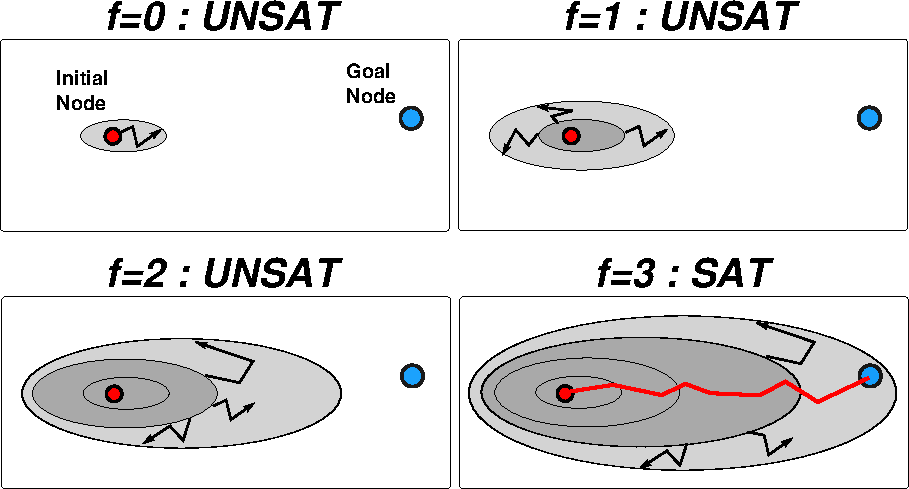
\includegraphics[width=0.8\linewidth]{img/astar/plateau-5.pdf}
 \caption{The concept of \astar as a sequence of satisficing searches.}
 \label{fig:astar-sat}
\end{figure}

%% Reduced as a result of compression
% One may notice the difference between the satisficing search and the search on a plateau.
% The former starts from a single initial node while the latter may start from multiple initial nodes.
% For example, in satisficing planning, the search space contains a single start node which corresponds to an initial state.
% % 
% In contrast, when \astar starts expanding a new current $f$ value $f_{\mit{cur}}$ after expanding all nodes with $f<f_\mit{cur}$,
% there may be multiple nodes with $f=f_\mit{cur}$ in the open list.
% These nodes are generated as a result of expansions of the parent nodes with $f<f_\mit{cur}$.
% % The search in this plateau terminates when the plateau is proven to contain no goal nodes (UNSAT), or some goal is found (SAT).
% % When the plateau is UNSAT, then the search continues to the next plateau.
% % 
% However, the difference is superficial: The latter can be reduced to the former case by introducing a dummy node
% which acts as a common parent of all initial nodes. We can thus reformulate the plateau search problem as a satisficing search from the single dummy node.

This is somewhat similar to the standard approach to model-based planning 
using SAT/IP/CP solvers \cite{kautz1992planning,van2005optiplan}, %avoid ''sequential'' here because it can refer to either the semantics (wrong) or to the solving strategy (correct)
% \cite{rintanen2012planning,   Rintanen is state-of-the-art but not a good exemplar for this point, because his solver jumps around various horizons. van2005optiplan} in a slightly different sense.  
based on an iterative strategy where a planning problem is converted to a corresponding constraint satisfaction problem with a finite horizon $t$ (plan length / makespan). The search starts from the horizon 0 and tests if the problem is satisfiable. If not, then it increases the horizon, add constraints excluding solutions below $t$, and retests the same problem with additional constraints for a new horizon $t+1$.

% The strategy of iterative search over a sequence of horizons in model-based planning is somewhat analogous to our view of \astar as a sequence of satisficing search over a set of plateaus.

%In forward heuristic search algorithms such as \astar, the concept of horizon corresponds to the $f$ value, which is a lower bound of the solution cost.

% XXX it's not a correct/safe to say that model-based methods solves from scratch on each iteration. In a model-based planners, at iteration  t, a constraint is added to exclude solutions with <t steps/layers (depending on whether layers are sequential/parallel) so that only possible solutions for that horizon are tested, so on the t't hiteration no search effort is wasted searching for solutions <t. This is different from the way IDA* repeats all work on each iteration.

%% A key difference in the \astar-based cost-optimal planning from the model-based planning is
%% that the information is transmitted between different horizons:
%% In \astar, nodes that are generated in the smaller
%% $f$ layer will be ``sent'' to the larger $f$ layer through the global OPEN
%% list, while current model-based methods prove the satisfiability of
%% different horizons independently -- in each iteration of the search,
%% they have to generate a new instance of a SAT/IP problem, and the
%% underlying model-based solvers are forced to start the search from the scratch.

%More precisely, each iteration of \astar only requires testing the satisfiability in the space of particular
%$f$ while each iteration of model-based solvers tests the satisfiability in the space of all nodes $0\leq f(n)\leq t$ ($t$: a horizon).   


%This latter behavior also connects model-based approaches to Iterative Deepening \astar
%\cite{korf1985depth} where the search is restarted from the scratch on each iteration, forgetting the past search
%effort in order to ensure the linear space usage.
%\refig{fig:idastar-sat} illustrates the concept.
% 
%\todo*{A more standard interpretation of the connectin between SAT/IP/CSP planning vs \astar is that SAT/IP/CSP are
%doing iterated deepening, where each iteration seeks a satisficing solution, like IDA*. }
% 

It is also reminiscent of the behavior of iterative deepening \astar \cite{korf1985depth}, which executes a series of satisficing searches with an $f$-cost limit which increases on each iteration. However, ``\astar-as a sequence of satisficing search'' differs from IDA* in that IDA*, in order to achieve linear memory usage, repeats previous work on each iteration. Instead of searching a particular plateau in each iteration, IDA* searches through the union of several plateaus.

% Unsurprisingly, this can also be modeled as sequence of satisficing searches (\refalgo{alg:idastar-sat}).
% 
% \begin{algorithm}
%  \begin{algorithmic}
%   \LOOP
%   \STATE Search $S=\bigcup_{0\leq f \leq F} \plateau{f}$ for any goal state
%   \IF{$S$ contains some goal}
%   \RETURN solution
%   \ELSE
%   \STATE Reset the internal state of the planner, increase $F$
%   \ENDIF
%   \ENDLOOP
%  \end{algorithmic}
%  \caption{IDA* as iterations of satisficing search on unions of plateaus}
%  \label{alg:idastar-sat}
% \end{algorithm}

%% \begin{figure}[htbp]
%%  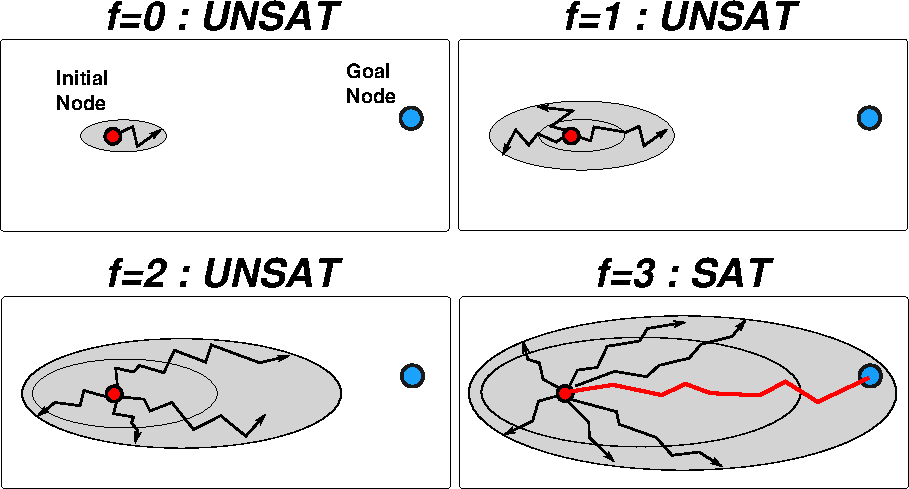
\includegraphics{img/astar/plateau-6.pdf}
%%  \caption{The concept of IDA* and model-based planning as a sequence of satisficing searches.}
%%  \label{fig:idastar-sat}
%% \end{figure}

The framework of ``\astar as a series of satisficing searches'' suggests that we can directly apply satisficing search techniques to optimal search using \astar, especially for each $f$-cost plateau search.
% 
In the following two subsections, as well as in the next section, we show that this framework  (1) provides a better understanding of depth-diversification (\refsec{sec:depth-vs-types}), (2) allows us to prove the completeness of \astar on infinite graph depending on the tie-breaking methods (\refsec{sec:completeness-on-infinite-space}), and (3) allows us to improve the performance of \astar on Zerocost domains (\refsec{sec:distance-to-go}).

\subsection{Depth Diversification as Satisficing Search}
\label{sec:depth-vs-types}
Within this framework, the implementation of depth diversification can be viewed as a variant of the Type-based diversification approach \cite{xie14type},  specifically tailored for Zerocost domains.

\citeauthor{xie14type} proposed \emph{type based buckets}, an implementation of the OPEN list which partitions the nodes into buckets according to some set of key values (\emph{types}). They proposed several types such as $\brackets{1}$, $\brackets{g}$, $\brackets{h}$ or $\brackets{g,h}$. At each type-based expansion, a randomly selected node from a randomly selected single bucket is selected. For example, with type $\brackets{g,h}$, a node with $g=5$ and $h=3$ is put into a bucket  $\brackets{5,3}$. This mechanism diversifies the search so that it tries to expand the nodes with various distances from the initial state and various distances from a goal state.

They then proposed Type-GBFS, which alternates the expansion between normal GBFS with a $[h,\fifo]$ sorting criteria and type-based expansion. This alternating framework addresses a weakness of GBFS: 
GBFS is solely guided by the heuristic function $h$, and heuristic errors in $h$ can easily misguide GBFS to spend all of its time in the wrong part of the search space -- GBFS can become trapped due to heuristic error and cannot recover from the wrong decision until expanding all nodes in that branch.
In the worst case, on infinite graphs, GBFS is not complete because it can be misdirected by the heuristic guidance forever \cite{Valenzano2016}.
In contrast, in Type-GBFS, the alternation with type-based expansion introduces exploratory behavior of nodes with low $g$ and high $h$, offering the possibility of escaping from heuristic error traps.
As a result, Type-GBFS is probabilistically complete on infinite graphs \cite{Valenzano2016}.

Type-GBFS was primarily evaluated in the context of satisficing search with no consideration of plan quality, and performance is solely evaluated according to coverage.
Thus, Xie et al adopted a unit-cost domain model: All action costs are ignored and replaced with unit costs in their experiments in order to boost coverage \cite{xie14type}. This is a commonly used technique for satisficing search which is also used in the first iteration of LAMA2011 \cite{richter2011lama}. 

% (i.e., finding either a goal node or exhausting the plateau)

In our framework of \astar as a sequence of satisficing searches, depth diversification after $h$ tie-breaking ($[f,h,\depth]$) can be viewed as the combination of (1) an implicit transformation of all 0-cost edges within a single $\plateau{f,h}$ to unit-cost edges, and (2) a pure type-based exploration within that plateau (unlike Type-GBFS, which alternates GBFS and type-based buckets).
 
The notion of \emph{depth} counts the number of 0-cost actions, which does not change the $f$ value and $h$
value, on the path from the entrance to the current plateau, to the current node.  Thus, 
depth-diversification treats  the problem of finding an exit from a particular plateau as a unit-cost satisficing search problem
-- the depth is analogous to a $g$-value which is calculated with unit costs and is restricted to a particular plateau.
%% Also, depth diversification puts the nodes in a particular depth into the corresponding depth bucket, then
%% diversifies the search among various depth buckets in a round-robin fashion (in this paper) or by a random
%% selection (conference version of this paper \cite{Asai2016}). If the depth corresponds to the unit-cost $g$-value
%% in each $\plateau{f,h}$, then the implementation-level mechanism for diversification is equivalent to
%% $\brackets{g}$, a type bucket of a single key value $g$. Thus, depth
%% diversification can be said to be using a type bucket of $\depth$ (modulo random/deterministic difference).

Depth diversification for tie-breaking in admissible \astar has a different purpose and context from Type-GBFS for satisficing search,
and differs as follows.
First, depth diversification  is focused on finding a satisficing plan \emph{within a single plateau} and on solving \emph{domains with 0-cost actions}.
% which is strictly harder than those without them. %worst-case complexity results for problem classes don't necessarily apply to specific instances, so using this ``strictly harder'' complexity result as justification is dangerous.
Therefore, depth diversification is applied after the sorting by $h$.
%Also, the role is limited to each plateau with the same $f$ and $h$ because nodes are put in the depth buckets only after being sorted by $f$ and $h$, 
In contrast, type buckets are global --- type buckets have no preceding sorting criteria, and all open nodes are stored in these buckets. Type-GBFS then alternates type buckets and sorting by $h$, not applying them in a cascade manner.

Nevertheless, the close relationship between depth diversification for admissible \astar and Type-GBFS for satisficing search is important. It shows that if we apply our framework of ``\astar as a series of satisficing searches'', we can directly use ideas which have been previously proposed for satisficing search within each $f$-cost plateau search.
% In the next section, we present another instance of this general approach.

\subsection{Completeness of \astar on an Infinite Graph}
\label{sec:completeness-on-infinite-space}

Similarly, we can use this framework for analyzing the completeness of \astar on infinite graphs with respect to various tie-breaking criteria.
First, \astar is complete on finite graphs regardless of the tie-breaking strategy \cite{hart1968formal}.
However, if the graph is infinite, the completeness of the algorithm depends on tie-breaking.
We consider several cases depending on which plateau is infinite.
 We only need to consider plateaus for $f \leq f^*$ because  \astar does not expand the nodes in $\plateau{f}$ for $f>f^*$.

\begin{defi}
 A graph is \emph{infinite} when the number of nodes in the graph has no upper bound.
\end{defi}

\begin{propo}
 \label{propo:f-less}
 If any $\plateau{f}$ for $f<f^*$ is infinite, then \astar does not terminate.
\end{propo}

\begin{proof}
 \refalgo{alg:astar-sat} requires proving the UNSAT-isfiability (that there is no solution) of all non-final plateaus, $\plateau{f}$ ($\forall f<f^*$), so if any of them are infinite, \astar does not terminate.
\end{proof}

The remaining cases assume that the following two conditions hold: 
 $\plateau{f}$ is finite  $\forall f<f^*$, and $\plateau{f^*}$ is infinite.
Under this assumption,
the completeness of \astar using tie-breaking $[f, \text{criterion}_2, \ldots \text{criterion}_k]$
depends on the completeness of the satisficing search algorithm corresponding to 
$[\text{criterion}_2, \ldots \text{criterion}_k]$ on $\plateau{f^*}$.
For the standard tie-breaking criteria, we can apply previously known results.

\begin{theo}[\citeauthor{Valenzano2016} \citeyear{Valenzano2016}]
 % [Probabilistic Completeness of $\varepsilon$-greedy node selection \cite{valenzano2014comparison}]
 $\varepsilon$-greedy node selection \cite{valenzano2014comparison} is \emph{probabilistically complete} on an infinite graph, i.e., 
 the probability of finding a solution
 % using $\varepsilon$-greedy node selection  \cite{valenzano2014comparison}
 approaches to 1 when the number of expansion $t$ approaches $\infty$.
\end{theo}

\begin{corollary}
 \astar with Random Order tiebreaking $[f,\ro]$ is probabilistically complete on an infinite graph
 when $\plateau{f}$ is finite for all $f<f^*$. %stating the conditions is not much longer than referencing conditions
 %satisfying the conditions in Proposition 2.
\end{corollary}

\begin{proof}
  $[f,\ro]$ is an instance of \astar using $[\ro]$ as a satisficing algorithm for plateau-search. Since $[\ro]$ is a special case of $\varepsilon$-greedy node selection with $\varepsilon=1$,
 $[\ro]$ is also probabilistically complete on an infinite $\plateau{f^*}$.
\end{proof}

Breadth-first search is complete when the graph has a finite branch factor below the solution depth.
Since FIFO tiebreaking $[f,\fifo]$ applies breadth-first search to $\plateau{f^*}$,  it follows that

\begin{propo}
 \astar with FIFO tiebreaking $[f,\fifo]$ is complete on an infinite graph when
 $\plateau{f}$ is finite  $\forall f<f^*$ and
 the maximum outdegree of the nodes is finite in $\plateau{f^*}$ below the solution depth.
\end{propo}

LIFO tie-breaking behaves equivalently to  a depth-first search with duplicate detection (DFS-dup) on $\plateau{f^*}$.
Assuming a fixed successor ordering, we get the following:

% \begin{proof}
%  % on an infinite graph is complete when (2) and (3) holds.
% % Since the solution have finite length and thus finite depth in the plateau, the search space expanded by FIFO (Breadth-first search) in infinite $\plateau{f^*}$ is finite.  Thus FIFO returns the solution in a finite time. 
% \end{proof}

\begin{propo} %corollary? (because dfs completeness is known under these conditions)
 \astar with LIFO tiebreaking $[f,\lifo]$ is complete on an infinite graph iff
 $\plateau{f}$ is finite for all $f\leq f^*$.
\end{propo}

%% \begin{proof}
%%  Completeness depends on the completeness of depth-first search on an infinite graph.
%%  On a graph satisfying (2), it has a possibility to search the infinitely large region.
%%  On a graph with (4) a finite maximum depth,
%%  it still has a possibility to search the infinitely large region in a subtree
%%  which does not contain the solution.
%%  If we assume both (2) and (4), then the graph becomes finite.
%% \end{proof}
\begin{proof}
 If $\plateau{f^*}$ is infinite, then
 either the maximum depth or the maximum outdegree of the nodes is infinite (has no upper bound).
 If the maximum depth has no upper bound,
 DFS-dup requires an arbitrary longer runtime before the first backtracking
 unless the solution is found before it.
 If the maximum outdegree has no upper bound,
 there is a successor ordering which forces DFS-dup
 to search all subtrees that do not contain solutions, and
 the size of the subtrees has no upper bound.
 If both the maximum depth and the maximum outdegree are finite, then $\plateau{f^*}$ is finite
 and DFS-dup is complete.
 Combined with \refpropo{propo:f-less},
 LIFO tie-breaking requires a finite $\plateau{f}$ for all $f\leq f^*$.
\end{proof}

Finally, we show the completeness of our iteration-based depth diversification in \refalgo{alg:depth}.

\begin{theo}
 \astar with Depth Diversification $[f,\depth,*]$ is complete % on an infinite graph % not necessary, as the following clause fully constrains the cases for which DD is complete
when  $\plateau{f}$ is finite  $\forall f<f^*$ and
 the maximum outdegree of the nodes is finite in $\plateau{f^*}$ for depths below the solution depth.
\end{theo}
 
\begin{proof}
 Any solution must have a finite depth $d^*$ on $\plateau{f^*}$.
 On every iteration of the $pop$ method of \refalgo{alg:depth} from the largest depth $D$ to the depth 0, each depth is expanded once.
 Since the maximum outdegree is finite,
 every node with depth $d\leq d^*$ will be expanded in a finite number of iterations.
\end{proof}

\begin{comment} % excessive and controversial claims
Despite all this, however, 
This the new view is so powerful that it unifies the two algorithms that have been developed separately for different purposes.
In the past, cost-optimal search techniques and satisficing search techniques used to be developed rather separately, and there has been only a handful of knowledge migration between them, most of which are abstract ideas such as delete-relaxation, landmarks, causal graphs or pattern database. % you seem to be claiming that these are not concrete algorithms, and that in contrast, \astar-as-series-of-satisficing-search allows direct import of concrete algorithms. However, as the type-gbfs vs depth comparison shows, the transfer is not trivial, and one can argue that the relationship between type-gbfs<g> vs depth is not much closer than the relationship between the FF heuristic and a pure admissible delete-relaxation heuristic.
Otherwise, the migration is unidirectional, in particular from cost-optimal to satisficing search, because it is easy or trivial to relax the optimality requirements.
% 
Our results and the new interpretation, \textbf{cost-optimal search is a sequence of satisficing searches on each plateau},
open up a new opportunity to break this boundary.
\end{comment}
% We provided the fundamentals of how and why we can import
% satisficing search techniques to the cost-optimal search (e.g. $\ffo$ heuristics in cost-optimal search).  There is a
% large avenue for future work in making a new migration happen.



\begin{comment}
% If you're still considering submitting tie-breaking for satisficing to a conference, including this subsection can block the conference paper and is a bad idea.
\subsection{Depth Diversification for Satisficing Search}

In order to strengthen the connection between tie-breaking and satisficing search,
we conducted another set of experiments. In the previous experiments, we showed that the distance-to-go
\ff heuristic $\ffo$ for \textbf{satisficing search within a plateau} was improved by the depth diversification
$\depth$.
% 
A natural extension of this idea is that the depth metric could also enhance the performance of $\ffo$ used for
\textbf{satisficing search in general}, which should hold if the search on plateaus and satisficing search are in
fact the same thing.
\todo*{``exporting from optimizing to satisficing'' and ``exporting from satisficing to optimizing'' are not symmetric. The latter is interesting and surprising, the former, not so much. --- changed the tone, emphasized the purpose}

We provide preliminary results on the 280 IPC8 satisficing track
instances. We tested GBFS using the distance-to-go variations of three
inadmissible heuristics for satisficing search: FF heuristics
 \cite{Hoffmann01}, Causal Graph (CG) heuristics \cite{Helmert2006}, and
Context Enhanced Additive (CEA) heuristics\ \cite{helmert2008unifying}.
For each heuristics, we tested eager and lazy search, with and without
the depth metric.  Tests are conducted under 5 min, 4GB
resource constraint.

In Eager search, depth metric
improved the performance of $\cgo$ ($60\rightarrow $ \textbf{64}), but no
improvement was observed in $\ceo$ ($62\rightarrow 62$)
and $\ffo$ ($73\rightarrow 73$). In Lazy search, depth metric
improved the performance of all three heuristics
($\cgo$: $36\rightarrow $ \textbf{50}, 
 $\ceo$: $39\rightarrow $ \textbf{48}, 
 $\ffo$: $54\rightarrow $ \textbf{93}). This is reasonable
because lazy search forces each node to derive the heuristic value from
its parent, and it makes more nodes to have the same heuristic value,
increasing the size of each plateau.

% \begin{table}[htbp]
%  \setlength{\tabcolsep}{0.3em}
%  \centering
%  \def\header{&\multicolumn{6}{c|}{Eager Search}&\multicolumn{6}{c|}{Lazy Search}\\}

\begin{center}
\begin{tabular}{|r|*{2}{*{3}{cc|}}}
\header & \(\ceo\) & \(\ceo\) & \(\cgo\) & \(\cgo\) & \(\ffo\) & \(\ffo\) & \(\ceo\) & \(\ceo\) & \(\cgo\) & \(\cgo\) & \(\ffo\) & \(\ffo\)\\
 & g & G & g & G & g & G & g & G & g & G & g & G\\
\hline
IPC8 & 62 & 62 & 60 & \textbf{64} & 73 & 73 & 36 & \textbf{50} & 39 & \textbf{48} & 54 & \textbf{93}\\
\hline
\end{tabular}
\end{center}

%  \caption{
%  Coverages under 5 min, 4GB experiments, comparing the variants with
%  and without depths. All configurations uses \fifo default
%  tie-breaking (we omit it from the description below).
%  $\ffo,\ceo,\cgo$ are the distance-to-go variations of FF,
%  Context Enhanced Additive, Causal Graph heuristics.
%  (g): GBFS with $[\hh]$ sorting strategy.
%  (G): GBFS with depth based diversification $[\hh,\depth]$.
%  }
%  \label{tbl:gbfs}
% \end{table}

% We also tested each combination on Type-GBFS, a recent \sota enhancement
% to GBFS. The results in \reftbl{tbl:type-gbfs} show that the depth
% metric also improves the performance of these configurations. Furthermore, we tested LAMA and
% Type-LAMA with and without depth metric. LAMA is an old \sota
% satisficing planner combining various satisficing enhancements such as
% Lazy-evaluation, distance-to-go estimates, multi-heuristic search and
% preferred operator queues. Type-LAMA is a newer \sota planner and an
% extension of LAMA using Type-GBFS, and it has performed the best among non-portfolio
% planners in IPC8 satisficing track. In \reftbl{tbl:lama}, we observed
% that the depth metric also improved the performance of LAMA and Type-LAMA.
% 
% \begin{table}[htbp]
%  \setlength{\tabcolsep}{0.3em}
%  \centering
%  \def\header{&\multicolumn{6}{c|}{Eager Search}&\multicolumn{6}{c|}{Lazy Search}\\}

\begin{center}
\begin{tabular}{|r|*{2}{*{3}{cc|}}}
\header & \(\ceo\) & \(\ceo\) & \(\cgo\) & \(\cgo\) & \(\ffo\) & \(\ffo\) & \(\ceo\) & \(\ceo\) & \(\cgo\) & \(\cgo\) & \(\ffo\) & \(\ffo\)\\
 & gt & Gt & gt & Gt & gt & Gt & gt & Gt & gt & Gt & gt & Gt\\
\hline
IPC8 & \textbf{57} & 55 & 76 & \textbf{79} & 80 & 79 & 44 & \textbf{53} & 66 & \textbf{74} & 66 & \textbf{92}\\
\hline
barman(20) & 0 & 0 & 0 & 0 & \textbf{4} & 2 & 0 & 0 & 0 & 0 & 0 & 0\\
cavediving(20) & 6 & 6 & 7 & 7 & 7 & 7 & 6 & 7 & 7 & 8 & 7 & 7\\
childsnack(20) & \textbf{2} & 0 & \textbf{3} & 0 & 0 & 0 & 2 & 1 & 6 & 5 & 2 & 2\\
citycar(20) & 4 & 5 & 1 & 1 & 3 & 3 & 1 & \textbf{9} & 0 & 0 & 0 & \textbf{7}\\
floortile(20) & 2 & 2 & 2 & 2 & 2 & 2 & 2 & 2 & 1 & 1 & 2 & 2\\
GED(20) & 0 & 0 & 8 & 9 & 16 & 15 & 0 & 0 & 11 & 11 & 15 & \textbf{17}\\
hiking(20) & 16 & 16 & 20 & 20 & 20 & 20 & 16 & 15 & 18 & 19 & 18 & 18\\
maintainance(20) & 16 & 16 & 16 & 16 & 13 & 13 & 7 & 7 & 7 & 7 & 9 & 10\\
openstacks(20) & 0 & 0 & 0 & 0 & 0 & 0 & 0 & 0 & 0 & 1 & 0 & \textbf{6}\\
parking(20) & 0 & 0 & 0 & 0 & 1 & 2 & 0 & 0 & 0 & 0 & 1 & \textbf{8}\\
tetris(20) & 1 & 1 & 13 & \textbf{15} & 2 & 2 & 1 & 3 & 9 & \textbf{15} & 2 & \textbf{4}\\
thoughtful(20) & 9 & 8 & 5 & 5 & 12 & 13 & 9 & 9 & 5 & 5 & 10 & 11\\
transport(20) & 1 & 1 & 1 & \textbf{4} & 0 & 0 & 0 & 0 & 2 & 2 & 0 & 0\\
visitall(20) & 0 & 0 & 0 & 0 & 0 & 0 & 0 & 0 & 0 & 0 & 0 & 0\\
\hline
\end{tabular}
\end{center}

%  \caption{
%  Coverages of Type-GBFS under 5 min, 4GB experiments, comparing the variants with
%  and without depths. All configurations uses \fifo default
%  tie-breaking (we omit it from the description below).
%  $\ffo,\ceo,\cgo$ are the distance-to-go variations of FF,
%  Context Enhanced Additive, Causal Graph heuristics.
%  In each expansion, Type-GBFS alternates standard GBFS and Type-based exploration using $[g,\hh]$.
%  The sorting strategy of the GBFS part of (gt) is $[\hh]$, while (Gt) uses $[\hh,\depth]$.
%  }
%  \label{tbl:type-gbfs}
% \end{table}
% 
% \begin{table}[htbp]
%  % \setlength{\tabcolsep}{0.1em}
%  \centering
%  \begin{center}
\begin{tabular}{|r|ll|ll|}
 &  &  &  & \\
 & LAMA & LAMA & Type-LAMA & Type-LAMA\\
 &  & + depth (\(\ffo\)) &  & + depth (\(\ffo\))\\
\hline
IPC8 & 111 & \textbf{125} & 112 & \textbf{117}\\
\hline
barman(20) & 8 & \textbf{10} & 9 & 8\\
cavediving(20) & 7 & 7 & 6 & 7\\
childsnack(20) & 0 & \textbf{10} & 2 & \textbf{6}\\
citycar(20) & 1 & 0 & 5 & 4\\
floortile(20) & 2 & 2 & 2 & 2\\
GED(20) & 20 & 20 & 20 & 20\\
hiking(20) & 15 & \textbf{17} & 15 & 15\\
maintainance(20) & 1 & 1 & 6 & 6\\
openstacks(20) & 17 & 17 & 15 & \textbf{17}\\
parking(20) & 9 & 9 & 6 & 6\\
tetris(20) & 2 & 2 & 2 & 1\\
thoughtful(20) & 14 & 15 & 14 & 15\\
transport(20) & 2 & 2 & 1 & \textbf{3}\\
visitall(20) & 13 & 13 & \textbf{9} & 7\\
\hline
\end{tabular}
\end{center}

%  
%  \caption{ Coverages of satisficing planners LAMA (winner of IPC7, old \sota)
%  and Type-LAMA (non-portfolio winner of IPC8, newer \sota) under 5 min, 4GB
%  experiments, comparing the performance between the original and the
%  depth-enhanced variants. All configurations run the first GBFS
%  iteration only, apply \fifo default tie-breaking (we omit it from
%  the description below), apply lazy evaluation and use distance-to-go synergy
%  heuristics $\ffo / \hat{h}^{\text{LMcount}}$.
%  % 
%  LAMA alternates between four OPEN lists: an open list of $[\ffo]$, a
%  preferred operator queue of $\ffo$, an open list of
%  $[\hat{h}^{\text{LMcount}}]$, and a preferred operator queue of
%  $\hat{h}^{\text{LMcount}}$.  In contrast, Type-LAMA alternates
%  between five OPEN lists: In addition to the 4 queues in LAMA, it has a
%  type-based exploration queue using $[g,\ffo]$.  The depth is applied
%  only to the first queue, i.e. $[\ffo] \rightarrow [\ffo,\depth]$, and
%  is not applied to the other queues. In both LAMA and Type-LAMA, depth
%  metric improves the coverage.}
%  \label{tbl:lama}
% \end{table}
\end{comment}

\begin{comment} % Too much excitement. We've already said enough already on this.
In the past, cost-optimal search techniques and satisficing search techniques used to be developed rather separately, and there has been only a handful of knowledge migration between them, most of which are abstract ideas such as delete-relaxation, landmarks, causal graphs or pattern database.
Otherwise, the migration is unidirectional, in particular from cost-optimal to satisficing search, because it is easy or trivial to relax the optimality requirements.
% 
Our results and the new interpretation, \textbf{cost-optimal search is a sequence of satisficing searches on each plateau},
open up a new opportunity to break this boundary.  We provided the fundamentals of how and why we can import
satisficing search techniques to the cost-optimal search (e.g. $\ffo$ heuristics in cost-optimal search).  There is a
large avenue for future work in making a new migration happen.
\end{comment}

